\begin{figure}[t]
\centering
\vspace{-1.cm}
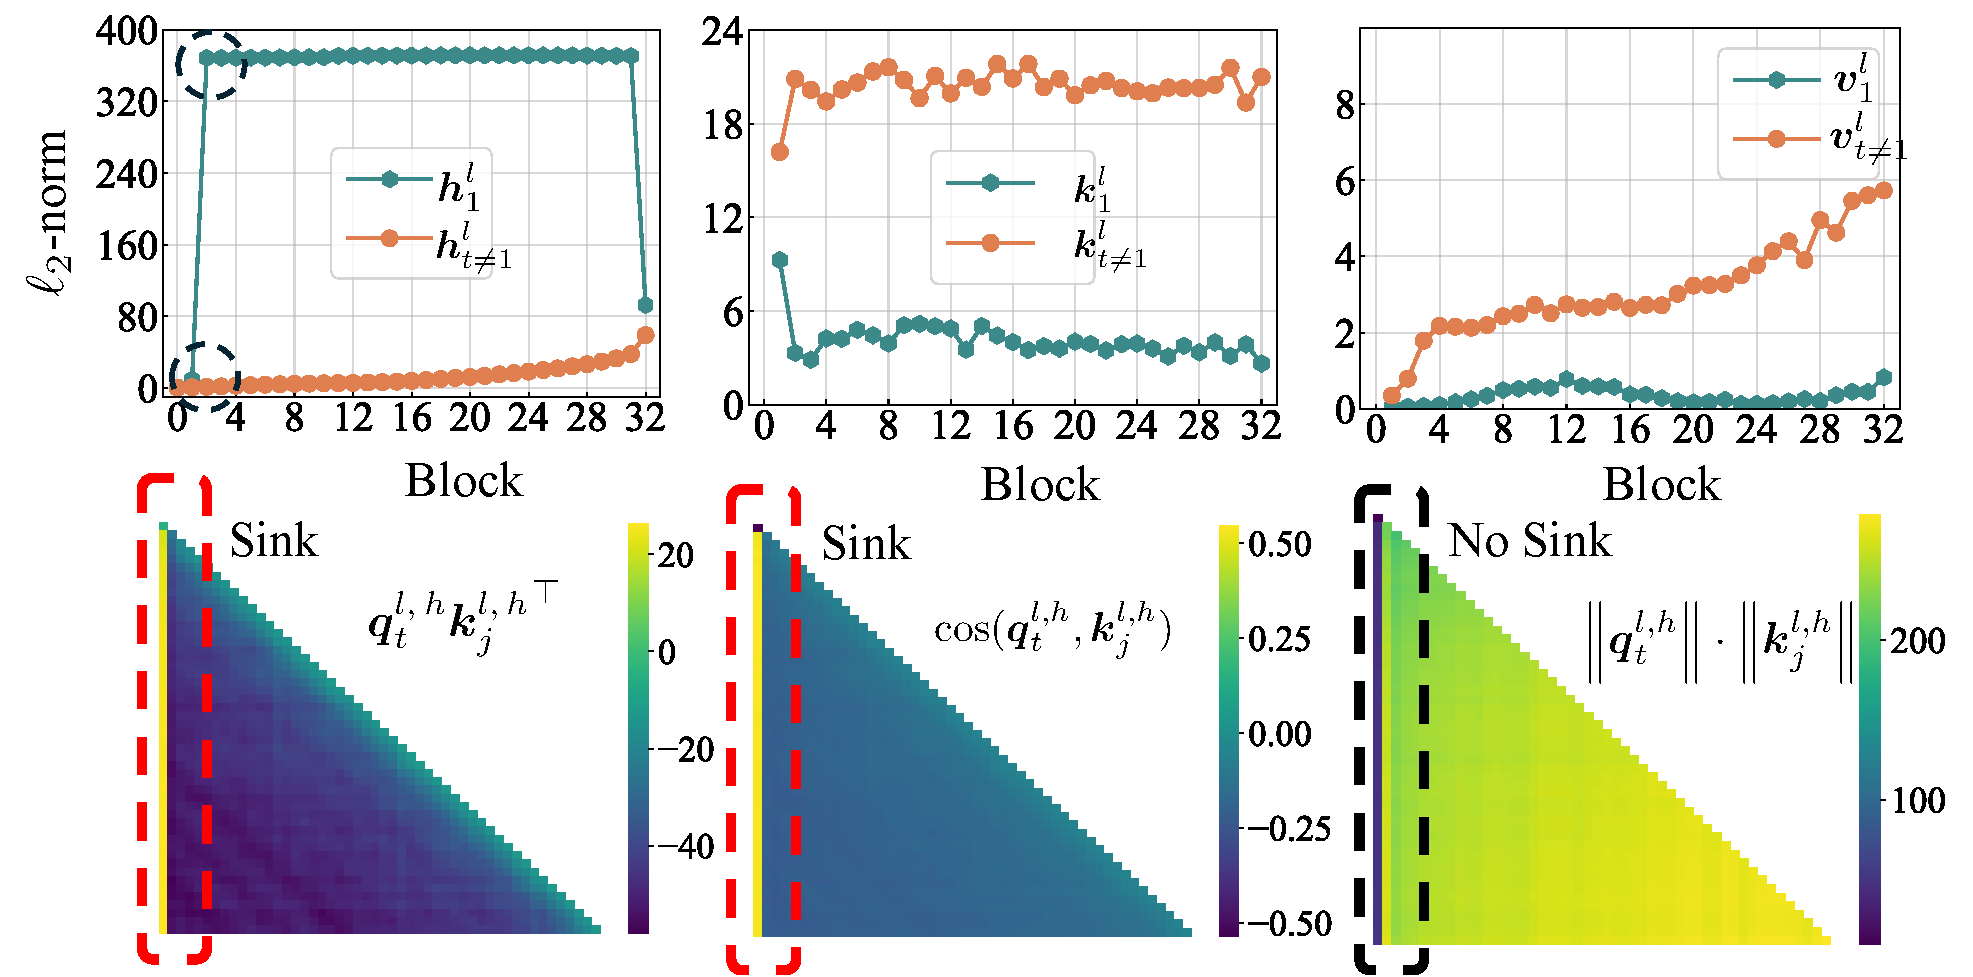
\includegraphics[width=\textwidth]{figures/activations_llama3-7b.pdf}
% \subfigure[]{\includegraphics[width=0.45\textwidth]{figures/domains_metric1.pdf}}
% \begin{subfigure}[htbp]{0.48\textwidth}
%     \centering
    
% \end{subfigure}
% \hfill
% \begin{subfigure}[htbp]{0.48\textwidth}
%     \centering
%     \includegraphics[width=\textwidth]{figures/Meta-Llama-3-8B_value_states.pdf}
% \end{subfigure}
\vspace{-0.3cm}
\caption{In LLaMA3-8B Base, (\emph{Top}) the first token has significantly larger $\ell_2$-norm of hidden states, but much smaller $\ell_2$-norm of keys and values than the mean of other tokens; (\emph{Bottom}) cosine similarity instead of norm product contributes to attention sink. We delay more visualizations to Appendix~\ref{vis_norm}.\looseness=-1
}
\label{massive}
\end{figure}

\vspace{-.2cm}
\section{Properties of attention sink}
\vspace{-.1cm}


\vspace{-.1cm}
\subsection{The first token acts as biases}\label{section3_1}
\vspace{-.1cm}
\textbf{Uniqueness of the first token.} It is noted that the calculation of hidden states for the first token has no involvement of self-attention $\boldsymbol{h}_1^{l}=\textrm{FFN}(\textrm{LN}(\boldsymbol{o}_1^l + \boldsymbol{h}_1^{l-1})) +  \boldsymbol{o}_1^l + \boldsymbol{h}_1^{l-1}$, where $\boldsymbol{o}_1^l=\textrm{LN}(\boldsymbol{h}_1^{l-1})\begin{bmatrix}
    \boldsymbol{W}^{l\textrm{,}1} & \boldsymbol{W}^{l\textrm{,}2} & \cdots & \boldsymbol{W}^{l\textrm{,}H}\\
\end{bmatrix}\boldsymbol{W}_{O}^l$. Therefore, $\boldsymbol{h}_1^l$, and corresponding queries/keys/values $\boldsymbol{k}_1^{l\textrm{,}h}=\textrm{LN}(\boldsymbol{h}_1^{l-1})\boldsymbol{W}_{K}^{l\textrm{,}h}$, $\boldsymbol{q}_1^{l\textrm{,}h}=\textrm{LN}(\boldsymbol{h}_1^{l-1})\boldsymbol{W}_{Q}^{l\textrm{,}h}$, $\boldsymbol{v}_1^{l\textrm{,}h}=\textrm{LN}(\boldsymbol{h}_1^{l-1})\boldsymbol{W}_{V}^{l\textrm{,}h}$ could be considered as the MLP output of input word embedding $\boldsymbol{x}_1\boldsymbol{W}_E$. Using LLaMA3-8B Base~\citep{dubey2024llama}, we show that from certain transformer block, e.g., $l=2$, the $\ell_2$-norm of $\boldsymbol{h}_1^l$ is significantly larger than that of other tokens $\boldsymbol{h}_{t\neq 1}$ in Figure~\ref{massive}(\emph{Top}). This reproduces massive activations in \citet{cancedda2024spectral,sun2024massive}. Despite the large $\ell_2$-norm of hidden states, we observe that the $\ell_2$-norm of keys and values of the first token is significantly smaller than that of other tokens in the same figure, which was also observed in \citet{devoto2024simple, guo2024attention}.\looseness=-1 


% attention sink is correlated to the \textit{massive activations} of hidden states $\boldsymbol{h}_1^l$ in LLMs. They showed that the hidden states of sink tokens, e.g., $\boldsymbol{h}_1^l$, typically exhibit huge magnitude in several dimensions. We observe that after the second transformer block, the $\ell_2$-norm of $\boldsymbol{h}_1$ is significantly larger than that of the mean of other tokens $\boldsymbol{h}_{t\neq 1}$. We further visualize the $\ell_2$-norm of keys and values in all transformer blocks. Counter-intuitively, both the $\ell_2$-norm of $\boldsymbol{k}_1^l$ and $\boldsymbol{v}_1^l$ (we take the mean value of all heads) are significantly smaller than other tokens from specific transformer block, e.g., $l=2$ for LLaMA3-8B Base.

\textbf{QK angles contribute to attention sink.}  In the $l$-th transformer block, we consider the keys and queries after adding PE (Rotary in LLaMA3-8B Base): $\boldsymbol{k}_t^{l\textrm{,}h}=\textrm{LN}(\boldsymbol{h}_t^{l-1})\boldsymbol{W}_{K}^{l\textrm{,}h}\boldsymbol{R}_{\Theta\textrm{,}\,-t}$, $\boldsymbol{q}_t^{l\textrm{,}h}=\textrm{LN}(\boldsymbol{h}_t^{l-1})\boldsymbol{W}_{Q}^{l\textrm{,}h}\boldsymbol{R}_{\Theta\textrm{,}\,-t}$, where LN is RMSNorm~\citep{zhang2019root}: $\textrm{LN}(\boldsymbol{h})=\frac{\boldsymbol{h}}{\textrm{RMS}(\boldsymbol{h})}\odot\boldsymbol{g}$ and $\textrm{RMS}(\boldsymbol{h})=\sqrt{\frac{1}{d}\sum_{i=1}^d\boldsymbol{h}_i^2}$.
% \looseness=-1 
% \begin{equation}
%     \textrm{LN}(\boldsymbol{h})=\frac{\boldsymbol{h}}{\textrm{RMS}(\boldsymbol{h})}\odot\boldsymbol{g}\textrm{,}\,\,\,\,\textrm{RMS}(\boldsymbol{h})=\sqrt{\frac{1}{d}\sum_{i=1}^d\boldsymbol{h}_i^2}\textrm{.}
% \end{equation}
Here $\boldsymbol{g}$ is a learnable gain parameter. Suppose that $\boldsymbol{h}_1^{l-1}$ already has massive activations. Since $\boldsymbol{h}_1^{l}$ has a massive magnitude in specific dimensions, the LN operation retains the magnitude in these dimensions and further reduces the magnitude in other dimensions, leading to that $\boldsymbol{q}_1^{l\textrm{,}\,h}$,  $\boldsymbol{k}_1^{l\textrm{,}\,h}$, and  $\boldsymbol{v}_1^{l\textrm{,}\,h}$ are distributed on different manifolds, especially for $\boldsymbol{k}_1^{l\textrm{,}\,h}$. 

For the $t$-th query, we know that $\boldsymbol{q}_t^{l\textrm{,}\,h}{\boldsymbol{k}_{1}^{l\textrm{,}\,h}}^\top$ typically has much larger values than $\boldsymbol{q}_t^{l\textrm{,}\,h}{\boldsymbol{k}_{j\neq 1}^{l\textrm{,}\,h}}^\top$, as visualized in Figure~\ref{massive}(\emph{Bottom}). We further show that due to the different manifold of $\boldsymbol{k}_1^{l\textrm{,}\,h}$, the angles between $\boldsymbol{k}_1^{l\textrm{,}\,h}$ and $\boldsymbol{q}_{t}^{l\textrm{,}\,h}$ play an important role. Considering $\boldsymbol{q}_t^{l\textrm{,}h}{\boldsymbol{k}_j^{l\textrm{,}h}}^\top=\|\boldsymbol{q}_t^{l\textrm{,}h}\|\cdot\|\boldsymbol{k}_j^{l\textrm{,}h}\|\cdot\textrm{cos}(\boldsymbol{q}_t^{l\textrm{,}h}\textrm{,}\,\boldsymbol{k}_j^{l\textrm{,}h})$, we visualize the cosine similarity between keys and values, and the product of $\ell_2$-norm between keys and values in Figure~\ref{massive}(\emph{Bottom}). Although $\|\boldsymbol{q}_t^{l\textrm{,}h}\|\cdot\|\boldsymbol{k}_1^{l\textrm{,}h}\|$ is comparatively small,  $\textrm{cos}(\boldsymbol{q}_t^{l\textrm{,}h}\textrm{,}\,\boldsymbol{k}_1^{l\textrm{,}h})$ is significantly large, leading to attention sink. This explains why attention sink exists despite the small $\ell_2$-norm of keys of the first token. To conclude,  the first token leverages its keys to act as biases, thus minimizing the angles between $\boldsymbol{k}_{1}^{l\textrm{,}\,h}$ and $\boldsymbol{q}_{t}^{l\textrm{,}\,h}$ and exhibiting attention sink.


% When computing the dot product $\boldsymbol{k}_1^{l\textrm{,}\,h}{\boldsymbol{q}_{t\neq 1}^{l\textrm{,}\,h}}^T$


% We hypothesize that these dimensions contribute to the small angles between $\boldsymbol{k}_1^{l\textrm{,}\,h}$ and $\boldsymbol{q}_{t\neq 1}^{l\textrm{,}\,h}$. To validate this, we visualize the cosine similarity between keys and values, and the product of $\ell_2$-norm between keys and values in Figure~\ref{massive}, considering $\boldsymbol{q}_i^{l\textrm{,}h}{\boldsymbol{k}_j^{l\textrm{,}h}}^T=\left\|\boldsymbol{q}_i^{l\textrm{,}h}\right\|\cdot\left\|\boldsymbol{k}_j^{l\textrm{,}h}\right\|\cdot\textrm{cos}(\boldsymbol{q}_i^{l\textrm{,}h}\textrm{,}\,\boldsymbol{k}_j^{l\textrm{,}h})$. It is observed that the cosine similarity between the query of other tokens and they key of the first token is the largest in each row. While $\ell_2$-norm product is the smallest, which emphasizes that the small angles between $\boldsymbol{k}_1^{l\textrm{,}\,h}$ and $\boldsymbol{q}_{t\neq 1}^{l\textrm{,}\,h}$ lead to attention sink. This has no conflicts with the small $\ell_2$-norm of keys of the first token.\looseness=-1


% \textbf{Attention sink in sliding window attention.} Despite our focus on vanilla casual attention, we also explore the property of attention sink in Mistral 7B, which adopts a sliding window attention. 


% different data domain/data length/multilingual 
\vspace{-0.15cm}
\subsection{Measuring attention sink}
\vspace{-0.05cm}

% $\sum_{i}{\boldsymbol{A}_h^{(l)}}_{i,k}\gg \sum_{i}{\boldsymbol{\hat{A}}_h^{(l)}}_{i,k}$


\begin{figure}[t]
\centering
\vspace{-1.cm}
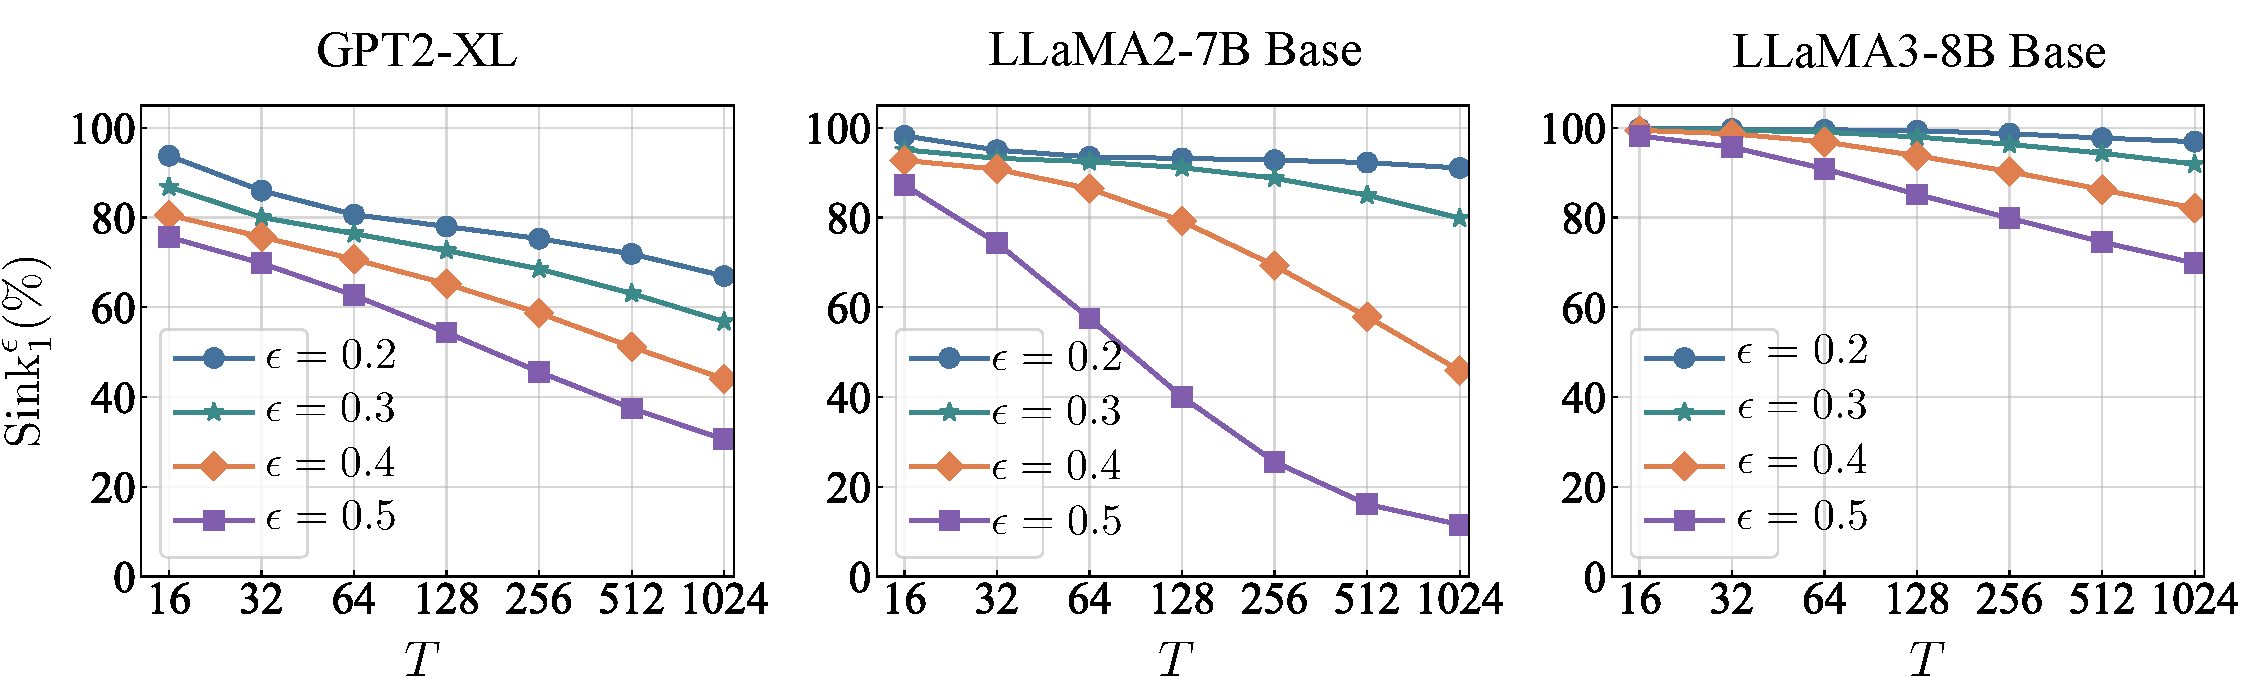
\includegraphics[width=\textwidth]{figures/metrics.pdf}
\vspace{-.6cm}
\caption{The metric $\textrm{Sink}_1^{\epsilon}$ (averaged on 100 sequences) tends to decrease with larger token lengths $T$. This tendency becomes more obvious with the more strict definition of attention sink (larger $\epsilon$).
}
\vspace{-0.2cm}
\label{metrics}
\end{figure}

% (\emph{Left}) GPT2-XL; (\emph{Middle}) LLaMA2-7B Base; (\emph{Right}) LLaMA3-8B Base. 

\textbf{Threshold-based metrics.} \citet{xiao2023efficient} showcased the appearance of attention sink by visualizing attention logits/scores in different heads/blocks. This leads to the intractability of measuring attention sink quantitatively due to the large number of attention heads and blocks. Therefore, we first explore the metrics to measure the attention sink. Within each head, we compute the importance scores for the $k$-th token $\alpha_k^{l\textrm{,}h}=\frac{1}{T-k+1}\sum_{i=k}^T \boldsymbol{A}_{i\textrm{,}\,k}^{l\textrm{,}\,h}$. We mainly focus on the first token $\alpha_1^{l\textrm{,}h}$. It is noted that $\frac{1}{T}\leq \alpha_1^{l\textrm{,}\,h}\leq 1$ since $\boldsymbol{A}_{1\textrm{,}\,1}^{l\textrm{,}\,h}=1$ and $0\leq \boldsymbol{A}_{i\neq 1\textrm{,}\,1}^{l\textrm{,}\,h}\leq 1$. Then we adopt a threshold-based metric, we consider a head has attention sink in the first token if $\alpha_1^{l\textrm{,}h}>\epsilon$. Considering that the whole model has $L$ blocks and each block has $H$ heads, we use the following metric to measure the attention sink of the whole LM: {\color{red!20!violet}$\textrm{Sink}_k^{\epsilon}=\frac{1}{L}\sum_{l=1}^L\frac{1}{H}\sum_{h=1}^H\mathbb{I}(\alpha_k^{l\textrm{,}h}>\epsilon)$}.\looseness=-1
% \looseness=-1
% \begin{equation}
%     \textrm{Sink}_k^{\epsilon}=\frac{1}{L}\sum_{l=1}^L\frac{1}{H}\sum_{h=1}^H\mathbb{I}(\alpha_k^{l\textrm{,}h}>\epsilon)
% \end{equation}




\textbf{Selections of thresholds.} Typically, the selections of thresholds represent the strictness of quantifying attention sink. Generally, a larger $\epsilon$ represents a strict definition for attention sink. There is no principal way to find an optimal threshold and we only use this metric to quantify the emergence of attention sink empirically. Based on Figure~\ref{metrics}, we prefer to select a threshold that is both strict in quantifying attention sink and less sensitive to the token length $T$. This gives us the selection of $\epsilon=\textrm{0.3}$. For fair comparisons, we need to fix $T$ when computing the metric, e.g., $T=\textrm{64}$. % we find that with a larger threshold $\epsilon$, our attention sink metric is more sensitive to the token length $T$.


% \textbf{Position-wise property.} With the definition of the attention sink metric, we quantitatively show that the attention sink always exists in the first token, not even the second token. 


% \begin{table}[t]
% \begin{center}
% \begin{tabular}{l|cc|cc}
% \toprule
% \multirow{2}{*}{LLM} & \multicolumn{2}{c}{w/ BOS} & \multicolumn{2}{c}{w/o BOS}\\
% & $\textrm{Sink}_1^{\epsilon}$(\%) & $\textrm{Sink}_2^{\epsilon}$(\%) &  $\textrm{Sink}_1^{\epsilon}$(\%) & $\textrm{Sink}_2^{\epsilon}$(\%) \\
% \midrule
% GPT2-XL  & 77.00 & 0.02 & 76.42 & 0.02 \\
% Llama2-7B Base & 92.47 & 0.00 & 92.11 & 19.54 \\
% Llama2-13B Base & 93.15 & 0.01 \\
% Llama3-8B Base & 99.47 & 0.00\\
% \bottomrule
% \end{tabular}
% \end{center}
% \vspace{-.2cm}
% \caption{Attention sink only appears in the first token, which is not strongly related to the BOS token.\looseness=-1}
% \vspace{-.2cm}
% \label{bos}
% \end{table}


% We consider the ratio between actual attention weights and averaged attention weights $\boldsymbol{A}^{l,h}_{i,k} / \boldsymbol{\hat{A}}^{l,h}_{i,k}$. Due to the ``vertical'' attention patterns of attention sink, we use $\frac{1}{T-k+1}\sum_{i=k}^T\boldsymbol{A}^{l,h}_{i,k} / \boldsymbol{\hat{A}}^{l,h}_{i,k}$ to represent the attention amplitude of $k$-th token when other tokens ``see'' this token. Since $ \boldsymbol{A}^{l,h}_{i,k}\leq 1$, the attention amplitude $\alpha_k^{l,h}=\frac{1}{T-k+1}\sum_{i=k}^T\boldsymbol{A}^{l,h}_{i,k} / \boldsymbol{\hat{A}}^{l,h}_{i,k}\leq (T+k) / 2$. Therefore, the range of $\alpha_k^{l,h}$ is highly depends on the values of $T$ and $k$. In this paper, we mainly discuss the scenario of $k=1$.



% \begin{figure}[t]
% \centering
% 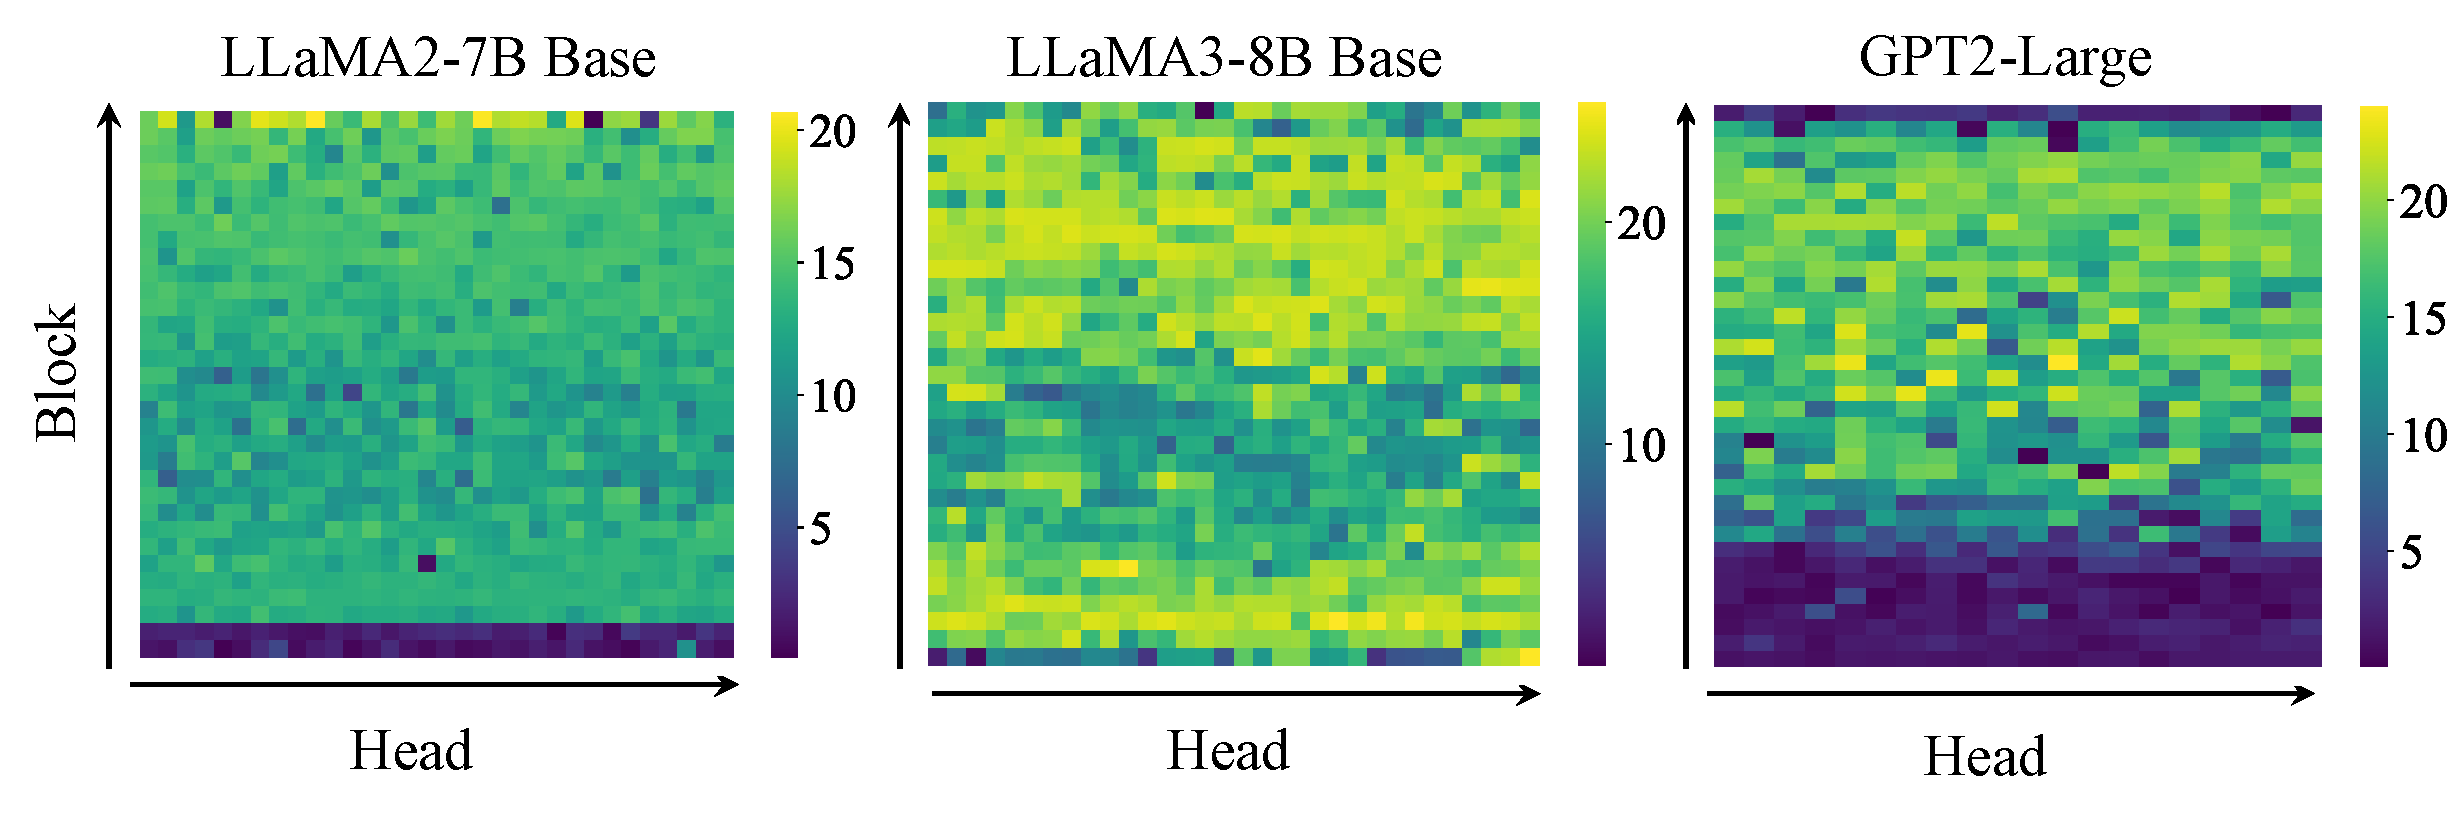
\includegraphics[width=\textwidth]{figures/head-layer.pdf}
% \caption{Attention amplitude of the first token $\alpha_1^{l\textrm{,}h}$ for different head IDs and block IDs in (\emph{Left}) LLaMA2-7B Base; (\emph{Middle}) LLaMA3-8B Base; (\emph{Right}) GPT2-Large. 
% }
% \vspace{-0.3cm}
% \label{head-layer}
% \end{figure}

% \textbf{Block-wise and head-wise property.} We first evaluate how attention amplitude $\alpha_1^{l\textrm{,}h}$ distributed in all heads and all blocks. To implement this, we sample over one hundred data inputs from the pile dataset~\citep{gao2020pile}. We select $T=50$ for simplicity and visualize the distributions of $\alpha_1^{l\textrm{,}h}$ across heads and blocks in pre-trained LLMs, as present in Figure~\ref{head-layer}. We notice that the attention sink has obvious layer-wise properties: the amplitude of the attention sink is relatively small in the initial layers while retaining large values in the middle layers. It is also noted that in the middle layers, there are still several heads that have no obvious attention sink.


% Due to the above properties, we propose to use $\max_{l} \sum_{h=1}^H\alpha_k^{l\textrm{,}h}$ as the metric for quantifying attention sink. 

% \begin{equation}
%     \max_{l} \sum_{h=1}^H\alpha_k^{l\textrm{,}h}
% \end{equation}

% \textbf{Position-wise property.} We find that the attention sink always exists in the initial token, not even the second token. Several literature~\citep{xiao2023efficient,cancedda2024spectral} consider that attention sink is strongly associated with the BOS token. However, we show that even without a BOS token, LLMs still exhibit initial-token attention sink except for Mistral-7B. 


% \begin{figure}[htbp]
% \centering
% % \subfigure[]{\includegraphics[width=0.45\textwidth]{figures/domains_metric1.pdf}}
% \begin{subfigure}[htbp]{0.48\textwidth}
%     \centering
%     \includegraphics[width=\textwidth]{figures/Llama-2-7b-hf_hidden_states.pdf}
% \end{subfigure}
% \hfill
% \begin{subfigure}[htbp]{0.48\textwidth}
%     \centering
%     \includegraphics[width=\textwidth]{figures/Llama-2-7b-hf_value_states.pdf}
% \end{subfigure}
% \vspace{-0.3cm}
% \caption{L2 norm of (\textit{Left}) the hidden states and (\textit{Right}) the values for Llama-2-7B model.
% }
% \label{lengths}
% \end{figure}



% Firstly, we consider a threshold-based metric following \citet{yu2024unveiling}: if $\alpha_k^{l,h}=\frac{1}{T-k+1}\sum_{i=k}^T\boldsymbol{A}^{l,h}_{i,k} / \boldsymbol{\hat{A}}^{l,h}_{i,k} > \epsilon$, $k$-th token is an attention sink in $l$-th layer $h$-th head. Then we consider the $k$-th token attention sink ratio in the whole model as $\alpha_k$. Alternatively, we consider another metric $\beta_k$ to compute the amplitude of attention sink in the model. In this paper, we mainly focus on the initial token attention sink ($k=1$).\looseness=-1
% \begin{equation}
%     \alpha_k=\frac{1}{L}\sum_{l}^L\frac{1}{H}\sum_{h}^H \mathbb{I}\left(\alpha_k^{l,h}>\epsilon\right)\textrm{,}\,\,\,\,\beta_k=\frac{1}{L}\sum_{l}^L\frac{1}{H}\sum_{h}^H \alpha_k^{l,h}\textrm{.}
% \end{equation}
    




% Specifically, we focus on the absolute value of attention score on the initial token $\boldsymbol{A}^{l,h}_{i,1}$ and its relative value $\boldsymbol{A}^{l,h}_{i,1}/\boldsymbol{\hat{A}^{(l)}}_{i,1}$. Notably, $1\leq i\leq T, 1\leq l\leq L, 1\leq h\leq H$. 

% Considering that previous literature has shown that initial token attention sink exists in most layers and heads, we 


\vspace{-0.2cm}
\subsection{Attention sink under different inputs}\label{section3_3}
\vspace{-0.2cm}

\textbf{Different data domains.} We first explore the effects of input domains on attention sinks. The pile dataset~\citep{gao2020pile}, a regular dataset for LM pretraining, has 17 available data domains. As shown in Appendix~\ref{vis_domains}, input domains have negligible effects on our attention sink metric $\textrm{Sink}_1^{\epsilon}$. 


% We sample 100 data inputs from each domain and evaluate the metric $\textrm{Sink}_1^{\epsilon}$.  No effects, see Appendix.\looseness=-1

% \begin{figure}[htbp]
% \centering
% % \subfigure[]{\includegraphics[width=0.45\textwidth]{figures/domains_metric1.pdf}}
% \begin{subfigure}[htbp]{0.48\textwidth}
%     \centering
%     \includegraphics[width=\textwidth]{figures/domains_metric1.pdf}
% \end{subfigure}
% \hfill
% \begin{subfigure}[htbp]{0.48\textwidth}
%     \centering
%     \includegraphics[width=\textwidth]{figures/domains_metric2.pdf}
% \end{subfigure}
% \caption{Attention distribution of token positions across various models.
% }
% \vspace{-0.3cm}
% \label{domains}
% \end{figure}

\textbf{Beyond natural languages.} We also consider two ideal scenarios: (i) randomly sample $T$ tokens from the tokenizer vocabulary $\mathbb{V}$ to construct a sequence and (ii) randomly sample 1 token from the tokenizer $\mathbb{V}$ and repeat it $T$ times. As present in Table~\ref{input}(\emph{Left}), attention sink still exists when the inputs are random tokens instead of natural language. However, with repeated tokens, attention sink in Mistral~\citep{jiang2023mistral} and LLaMA models disappears. In Appendix~\ref{explain_pe}, we prove that for LMs with NoPE/relative PE/ALiBI/Rotary, if the first $T$ tokens are the same, their corresponding hidden states are the same. They all have massive activations, thus dispersing the attention sink. We also provide the closed form/upper bound for attention scores in these LMs through Propositions~\ref{prop1}-\ref{prop4}.\looseness=-1

% In Appendix, we show that this phenomenon is related to the PE choices. For learnable PE in GPT2, attention sink is highly related to the PE in the first position.

\begin{table}[t]
\vspace{-1.1cm}
\caption{(\emph{Left}) Even with random sequence as input, there still exists an obvious attention sink. But with repeated tokens, the attention sink disappears for Mistral/LLaMA models. (\emph{Right}) Chat models have comparable attention sink metrics with base models.}
\vspace{-0.2cm}
\begin{minipage}[t]{0.54\linewidth}
\begin{center}
\begin{tabular}{l|ccc}
\toprule
\multirow{2}{*}{LLM} & \multicolumn{3}{c}{$\textrm{Sink}_1^{\epsilon}$(\%)} \\
& natural & random & repeat\\
\midrule
GPT2-XL  & 77.00 & 70.29 & 62.28 \\
Mistral-7B &  97.49 & 75.21 & \,\,\,0.00 \\
LLaMA2-7B Base & 92.47 & 90.13 & \,\,\,0.00 \\
LLaMA3-8B Base & 99.02 & 91.23 & \,\,\,0.00\\
\bottomrule
\end{tabular}
\end{center}
\end{minipage}
\hfill
\begin{minipage}[t]{0.40\linewidth}
\begin{center}
\begin{tabular}{l|cc}
\toprule
\multirow{2}{*}{LLM} & \multicolumn{2}{c}{$\textrm{Sink}_1^{\epsilon}$(\%)} \\
& Base & Chat\\
\midrule
Mistral-7B & 97.49 & 88.34 \\
LLaMA2-7B & 92.47 & 92.88 \\
LLaMA2-13B & 91.69 & 90.94 \\
LLaMA3-8B & 99.02 & 98.85\\
\bottomrule
\end{tabular}
\end{center}
\end{minipage}
\vspace{-.3cm}
\label{input}
\end{table}

\begin{figure}[t]
\centering
\begin{subfigure}[t]{\textwidth}
    \centering
    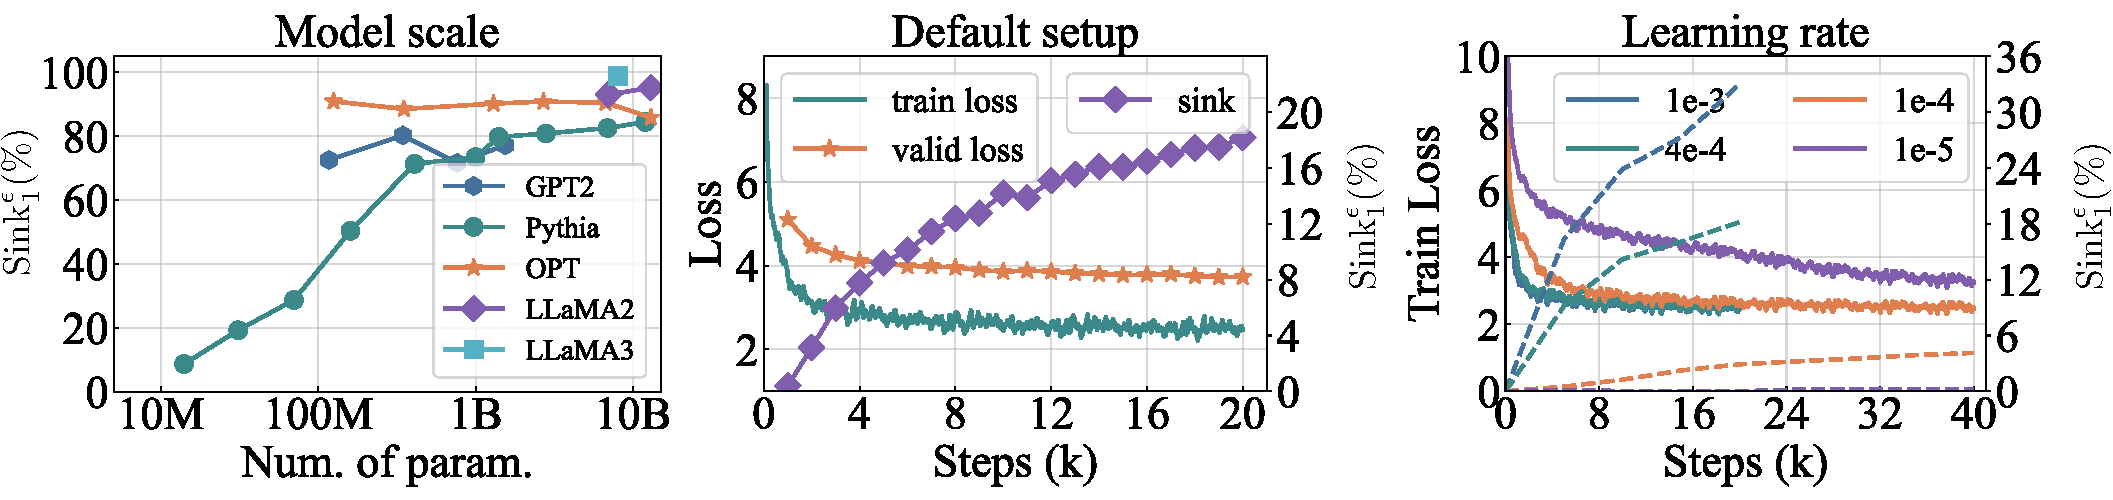
\includegraphics[width=\textwidth]{figures/model_scale.pdf}
\end{subfigure}
% \subfigure[]{\includegraphics[width=0.32\textwidth]{figures/domains_metric1.pdf}}
% \begin{subfigure}[t]{0.32\textwidth}
%     \centering
%     \includegraphics[width=\textwidth]{figures/tinyllama_loss.pdf}
% \end{subfigure}
% \hfill
% \begin{subfigure}[t]{0.32\textwidth}
%     \centering
%     \includegraphics[width=\textwidth]{figures/tinyllama_data.pdf}
% \end{subfigure}
\vspace{-0.675cm}
\caption{(\textit{Left}) Attention sink also emerges in small LMs. (\textit{Middle}) Dynamics of train/valid loss and $\textrm{Sink}_1^\epsilon$ during LM pre-training under the default setup. Attention sink emerges after certain optimization steps. (\textit{Right}) Training loss (solid lines)/attention sink (dashed lines) dynamics of LMs using different learning rates. We observe that with smaller learning rates, attention sink tends to emerge after more optimization steps and be less obvious.\looseness=-1}
\vspace{-0.2cm}
\label{model}
\end{figure}

\vspace{-0.3cm}
\subsection{Attention sink under different LMs}\label{section3_4}
\vspace{-0.2cm}
\textbf{Base vs. chat model.} Compared with base models, chat models are typically continually trained through instruction tuning~\citep{ouyang2022training}. From Table~\ref{input}(\emph{Right}), instruction tuning has an insignificant impact on attention sink, which motivates us to focus on the LM pre-training.\looseness=-1

\textbf{Model scale.} We evaluate the metric $\textrm{Sink}_1^{\epsilon}$ of LLaMA2 Base~\citep{touvron2023llama}, LLaMA3 Base~\citep{dubey2024llama}, Pythia~\citep{biderman2023pythia}, GPT2~\citep{radford2019language}, OPT~\citep{zhang2022opt} families. As visualized in Figure~\ref{model}(\emph{Left}), attention sink emerges in small LMs, even in Pythia-14M. Only in Pythia family, larger-sized LMs tend to have more obvious attention sink.\looseness=-1

% \textbf{Block-wise and head-wise property.} We visualize distributions of attention sink across different blocks and heads in LLaMA2/LLaMA3/GPT2/Mistral/Pythia/OPT family in Appendix~\ref{vis_domains}. We find that (i) though different LMs may have different distributions, they tend to have less attention sink heads in the earlier blocks; (ii) instruction tuning does not significantly modify such distribution.\looseness=-1
% \textbf{Block-wise and head-wise property.} Different LLMs have different block-wise and head-wise distributions. See Appendix.



% \begin{theorem}\label{theorem1}
% Suppose $f_{\theta}$ has no positional embeddings, if all the input tokens are the same $\boldsymbol{x}_t=\boldsymbol{x}, \forall\,\, 1 \leq t \leq T$, then the hidden states for all tokens are the same $\boldsymbol{h}_t^l=\boldsymbol{h}^l, \forall\,\, 1 \leq t \leq T, 1 \leq l \leq L$. Furthermore, there is no attention sink as $\boldsymbol{A}^{l,h}=\hat{\boldsymbol{A}}^{l,h}$. 
% \end{theorem}

% Theorem~\ref{theorem1} can be proved through mathematical induction, presented in the Appendix. It indicates that without positional embedding, no attention sink is guaranteed under the scenario that input tokens are the same. 


% \begin{corollary}\label{corollary1}
% Suppose $f_{\theta}$ has relative positional embeddings, including T5's relative PE, ALiBi, Rotary, and the first $T$ input tokens are the same $\boldsymbol{x}_t=\boldsymbol{x}, 1 \leq t \leq T$, then the hidden states for all tokens are the same $\boldsymbol{h}_t^l=\boldsymbol{h}^l, \forall\,\, 1 \leq t \leq T, 1 \leq l \leq L$. Furthermore, there is no attention sink.
% \end{corollary}

% For each domain, we report the mean values $\boldsymbol{\alpha}=\frac{1}{L\cdot H \cdot T}\sum_{l,h,i}\boldsymbol{A}^{(l)}_{i,1}/\boldsymbol{\hat{A}^{l}}_{i,1}$ and $\boldsymbol{\beta}=\frac{1}{L\cdot H \cdot T}\sum_{l,h,i}\boldsymbol{A}^{l,h}_{i,1}$.  


% \subsection{Attention Sink Under Different Input Lengths}

% \textbf{Different Token numbers.} We sample 10 data from each domain and combine them as our evaluation set. To evaluate the sensitivity of metrics of input token numbers, 

% we compute $\alpha_1$ and $\beta_1$ under different token numbers ($T$).


% \textbf{Beyond context window.} Typically, the context window of pretrained LLMs is 2k or 4k. We are wondering whether the initial token attention sink still exists beyond the context window. 




% \citet{xiao2023efficient} attributed this scenario to that the initial tokens are visible to all subsequent tokens. 

% \subsection{Attention Sink under Different Models}

% \textbf{Different model scales.} 


% \begin{figure}[htbp]
% \centering
% % \subfigure[]{\includegraphics[width=0.45\textwidth]{figures/domains_metric1.pdf}}
% \begin{subfigure}[htbp]{0.48\textwidth}
%     \centering
%     \includegraphics[width=\textwidth]{figures/models_metric1.pdf}
% \end{subfigure}
% \hfill
% \begin{subfigure}[htbp]{0.48\textwidth}
%     \centering
%     \includegraphics[width=\textwidth]{figures/models_metric2.pdf}
% \end{subfigure}
% \vspace{-0.3cm}
% \caption{Attention distribution of token positions across various models.
% }
% \label{lengths}
% \end{figure}

% \textbf{Base model vs. Chat model.}

% \begin{table}[t]
% \begin{center}
% \begin{tabular}{l|cc|cc}
% \toprule
% \multirow{2}{*}{LLM} & \multicolumn{2}{c}{$\alpha_1$ (\%)} & \multicolumn{2}{c}{$\beta_1$} \\
% & base & chat & base & chat \\
% \midrule
% Llama2-7B & 93.15 & 93.34 & 12.54 & 12.66\\
% Llama2-13B & 94.34 & 93.09 &  19.44 & 19.20\\
% Llama3-8B & 99.46 & 99.39 & 18.67 & 18.70\\
% Llama3.1-8B & 99.44 & 99.47 & 18.67 & 18.68\\
% \bottomrule
% \end{tabular}
% \end{center}
% \vspace{-.2cm}
% \caption{Memorization ratios (\%) of different values of (left) weight decay; (right) EMA.}
% \vspace{-.2cm}
% \label{tbl_decay_ema}
% \end{table}



% \textbf{}

% \subsection{Attention Sink Under Different LLMs}

% \textbf{Model scale.}

% \textbf{Base vs. chat models.}

% \textbf{Layer-wise property.}


% \textbf{Attention sink always exists in the first token, not even the second one.}

% \textbf{Attention sink can also happen in other positions.}


% \textbf{Attention sink is not associated with the BOS token.}


% \textbf{Attention sink exhibits layer-wise property.}



% Inspired by \citet{yu2024unveiling}, we define the following metric to measure the amplitude of attention weights\looseness=-1

% \begin{equation}
%     \boldsymbol{\alpha}=\frac{1}{H}\frac{1}{L}\sum_{h=1}^H\sum_{l=1}^L\frac{1}{T-k+1}\sum_{i=k}^T\frac{{\boldsymbol{A}_h^{(l)}}_{i,k}}{{\boldsymbol{\hat{A}}_h^{(l)}}_{i,k}}\textrm{.}
% \end{equation}
% Typically, $\boldsymbol{\alpha}_{k}$ is close to $1$ considering the average attention weights. 

% Alternatively, we consider the following metric 


% As preliminary experiments, we measure the amplitude attention weights of mainstream LLMs, including LLaMA family, GPT2, Pythia family, and OPT family.  


% \begin{figure*}[t]
% \centering
% \subfigure{\includegraphics[width=0.23\textwidth]{figures/visuals/Llama-2-7b-hf/token_len200_probe3.png}}
% \subfigure{\includegraphics[width=0.23\textwidth]{figures/visuals/Llama-2-7b-chat-hf/token_len200_probe3.png}}
% \subfigure{\includegraphics[width=0.23\textwidth]{figures/visuals/Llama-2-13b-hf/token_len200_probe3.png}}
% \subfigure{\includegraphics[width=0.23\textwidth]{figures/visuals/Llama-2-13b-chat-hf/token_len200_probe3.png}}
% \subfigure{\includegraphics[width=0.23\textwidth]{figures/visuals/Meta-Llama-3-8B/token_len200_probe3.png}}
% \subfigure{\includegraphics[width=0.23\textwidth]{figures/visuals/Meta-Llama-3-8B-Instruct/token_len200_probe3.png}}
% \subfigure{\includegraphics[width=0.23\textwidth]{figures/visuals/Meta-Llama-3.1-8B/token_len200_probe3.png}}
% \subfigure{\includegraphics[width=0.23\textwidth]{figures/visuals/Meta-Llama-3.1-8B-Instruct/token_len200_probe3.png}}
% \subfigure{\includegraphics[width=0.23\textwidth]{figures/visuals/gpt2-small/token_len200_probe3.png}}
% \subfigure{\includegraphics[width=0.23\textwidth]{figures/visuals/gpt2-medium/token_len200_probe3.png}}
% \subfigure{\includegraphics[width=0.23\textwidth]{figures/visuals/gpt2-large/token_len200_probe3.png}}
% \subfigure{\includegraphics[width=0.23\textwidth]{figures/visuals/gpt2-xl/token_len200_probe3.png}}
% \subfigure{\includegraphics[width=0.23\textwidth]{figures/visuals/opt-350m/token_len200_probe3.png}}
% \subfigure{\includegraphics[width=0.23\textwidth]{figures/visuals/opt-1.3b/token_len200_probe3.png}}
% \subfigure{\includegraphics[width=0.23\textwidth]{figures/visuals/opt-2.7b/token_len200_probe3.png}}
% \subfigure{\includegraphics[width=0.23\textwidth]{figures/visuals/opt-6.7b/token_len200_probe3.png}}
% \subfigure{\includegraphics[width=0.23\textwidth]{figures/visuals/pythia-410m/token_len200_probe3.png}}
% \subfigure{\includegraphics[width=0.23\textwidth]{figures/visuals/pythia-1b/token_len200_probe3.png}}
% \subfigure{\includegraphics[width=0.23\textwidth]{figures/visuals/pythia-2.8b/token_len200_probe3.png}}
% \subfigure{\includegraphics[width=0.23\textwidth]{figures/visuals/pythia-6.9b/token_len200_probe3.png}}
% \caption{Attention distribution of token positions across various models.
% }
% \vspace{-0.35cm}
% \label{fig:attention_dist}
% \end{figure*}

% by sampling $100$ prompts from the validation set and $100$ prompts from widely adopted downstream NLP tasks. 



% \begin{figure*}[t]
% \centering
% \subfigure{\includegraphics[width=0.32\textwidth]{figures/visuals/LLaMA2/token_len200_probe3_layer.png}}
% \subfigure{\includegraphics[width=0.32\textwidth]{figures/visuals/LLaMA3/token_len200_probe3_layer.png}}
% \subfigure{\includegraphics[width=0.32\textwidth]{figures/visuals/GPT2/token_len200_probe3_layer.png}}
% \subfigure{\includegraphics[width=0.32\textwidth]{figures/visuals/OPT/token_len200_probe3_layer.png}}
% \subfigure{\includegraphics[width=0.32\textwidth]{figures/visuals/Pythia/token_len200_probe3_layer.png}}
% \caption{Layer-wise property of first-token attention sink across various models.
% }
% \vspace{-0.35cm}
% \label{fig:layer}
% \end{figure*}

% \citet{yu2024unveiling} categorized attention sink tokens into initial tokens and non-initial high attention tokens. However, the initial token consistently has the attention sink while other non-initial high-attention tokens have no such position association, as shown in both \citet{yu2024unveiling} and Appendix. 


% Moreover, \citet{yu2024unveiling} claimed that the initial token is highly associated with the begin of sequence (BOS) token <s>. However, we find that even without a BOS token, the first token still has an attention sink. 


% Since our objective is to research on the properties and influential factors of attention sink, we first define how to detect and measure attention sink. 

% We would like to first show the universality of attention sink across different data inputs and LLMs. Specifically, we 








% \begin{table}[htbp]
% \begin{center}
% \caption{Summary of Large Language Models.}
% \begin{tabular}{l|l|l}
% \toprule
% LLM & Positional Embedding & BOS \\
% \midrule
% Pythia family & Rotary & No \\
% GPT2 family & Learnable & No \\
% LLaMA2, LLaMA3 families & Rotary & Yes \\
% Codellm 1B Nope & None & Yes\\
% Codellm 1B Rotary & Rotary & Yes\\
% Codellm 1B ALiBi & ALiBi & Yes\\
% \bottomrule
% \end{tabular}
% \end{center}
% \label{llms}
% \end{table}

% \subsection{Multiple datasets}

% Sciq, lamabada openai dataset

% \subsection{Multiple languages}

% \subsection{Multiple contexts}